\documentclass{article}

%% https://tex.stackexchange.com/a/38608
\usepackage{tkz-graph}
\usetikzlibrary{shapes.geometric}

\usepackage{amsmath, amssymb}
\usepackage{mathtools}
\usepackage{xcolor}
\usepackage{textcomp}

\usepackage{array}
\newcolumntype{L}{>{$}l<{$}} % math-mode version of "l" column type
\newcolumntype{C}{>{$}c<{$}} % math-mode version of "c" column type
\newcolumntype{R}{>{$}r<{$}} % math-mode version of "r" column type

%% Do not mess with this.
\usepackage[backend=bibtex,sorting=none,style=numeric-comp]{biblatex} 
\addbibresource{citation.bib}

\DeclarePairedDelimiter\abs{\lvert}{\rvert}%
\DeclarePairedDelimiter\norm{\lVert}{\rVert}%

\makeatletter

\let\oldabs\abs
\def\abs{\@ifstar{\oldabs}{\oldabs*}}

\let\oldnorm\norm
\def\norm{\@ifstar{\oldnorm}{\oldnorm*}}

\makeatother

\begin{document}

\title{\vspace{-8em}EECS 442: Final project\vspace{-1em}}
\author{James Starkman, jas497}
\date{\vspace{-1ex}Due 2017-05-03, submitted 2017-05-05\vspace{-2em}}
\maketitle

\section{Problem}

\subsection{Background and problem statement}

Businesses, especially large Internet-based ones, often want to analyze customer
behavior in order to better serve their customers' interests, and of course to
make more money while doing so.  One such company is Expedia, a multi-billion
dollar travel reservations and booking company.  It owns many brands, including
(but not limited to) Expedia.com, Hotels.com, trivago, Orbitz, and Travelocity,
with the latter three being relatively recent acquisitions.  Every year,
enormous numbers of people use Expedia-owned sites to search for hotels,
flights, and more at various destinations around the world.  Recently, Expedia's
data division made a sizeable (10.9M rows) dataset available.  The dataset
covers a subset of search history data for anonymized users of the Expedia.com
(US and generic), Expedia.ca (Canada), and Expedia.de (Germany) sites.  The
dataset is discussed in much more detail in the following section, but a few
important details are given here.  For example, the two-gigabyte dataset only
pertains to hotel searches made from the above three websites over the course of
the year 2015.  The fields logged include every field present on the Expedia
website, as well as information about the hotel, including broad categories
describing it.  Additionally, a binary field identifying whether the user is
using a mobile phone or not is logged, as well as whether or not the user
ultimately booked that particular hotel.  It is these two fields that shall form
the motivating question of this study: to what extent does mobile phone usage
cause booking rates?

\subsection{Symbol table}

In this study, the following symbols will be used.  They generally follow those
used by Hernan and Robins \cite{hernan2010causal} in their not-quite-published
work, \emph{Causal Inference} (the course textbook).

\begin{center}  
  \begin{tabular}{Ll}
    \text{Let} & be \\
    \hline
    A & 1 if the user was on a mobile device else 0 \\
    Y & 1 if the user made a booking else 0 \\
    L & a vector of covariates, discussed below \\
    \vec{l} & a given row's values for $L$\\
  \end{tabular}
\end{center}

\section{Data set} %%%%%%%%%%%%%%%%%%%%%%%%%%%%%%%%%%%%%%%%%%%%%%%%%%%%%%%%%%%%%

\subsection{Data source}

The dataset used in this report was released by Expedia in early April 2017 for
the American Statistical Association's annual Datafest event.  It consists of
two files, a two-gigabyte file and a hundred-megabyte file.


The larger file covers a subset of search history data for anonymized users of
the Expedia.com, Expedia.ca, and Expedia.de sites, as mentioned in the problem
definition above.  The file is structured as tab-separated values with
twenty-seven columns and almost eleven million rows.  The columns of this file
include: a timestamp (to the nearest minute); which site generated the record;
the user's country, region, city, and (if available) the (latitude, longitude)
pair and the distance between the user's location and the hotel's location; a
user ID number; whether the user accessed the site from a mobile device or
otherwise; whether the user was looking for package deals (paying for the hotel
and the airfare in the same booking); the ID of a marketing channel; the search
parameters (checkin, checkout, number of adults, number of children, number of
hotel rooms, and the ID of the destination); the country where the hotel is;
whether this viewing of a hotel resulted in a booking; the ID of the hotel;
details about the hotel (whether or not it is part of a major chain
(``branded''), average star rating by Expedia users on a five-point scale);
general ``bands'' into which the hotel falls (with regard to distance, price,
and popularity); and the number of similar events in the user's session.  The
bands are structured as enumerated types of five values, and have semantic
meanings of very low, low, middle, high, and very high.


Unlike the larger file, the smaller file does not contain raw data; rather, it
contains Expedia's estimates of how likely users would be to recommend different
destinations for different categories of things to do at the different
destinations.  These values are stored as the base-ten logarithm of the
estimated values, which helps compress the wide range of values that the
probability can take on.  These data are less suited to causal inference than
the data present in the larger file and have been ignored for this report.


Finally, it should be noted that bookings ($Y=1$) are in reality a rare event.
To accomodate for this, as well as to obscure their conversion rate, Expedia
deliberately included in the dataset a higher percentage of rows where $Y=1$
than there should be.  For example, if one na\"{\i}vely divides the sum of the
full \texttt{is-booking} column by the number of rows in that column, one finds
that about ten percent of clicks on listings resulted in bookings.  This
impossibly high value should not be taken literally.  Accordingly, any
statistical methods relying on the ratio between $Y=1$ and $Y=0$ cannot be used,
or at least, cannot be used to draw conclusions about Expedia's business.

\subsection{Chosen variables}

%% L = these:
%% user_location_country == hotel_country
%% is_package
%% srch_co - srch_ci
%% srch_adults_cnt
%% srch_children_cnt
%% srch_rm_cnt
%% prop_is_branded
%% prop_starrating
%% distance_band
%% hist_price_band
%% popularity_band

For this report, not all of the columns mentioned above were used.  This is due
to various reasons.  A common reason is that ID numbers are effectively
meaningless on their own.  The three user location columns (latitude, longitude,
and distance) were often null, resulting in their being eliminated from
consideration.  There are many possible locations, so more granular analyses
might violate positivity; to avoid that, location is only used as a binary
variable telling whether the country in which the user is located matches tthe
hotel's country (1) or not (0).  Similarly, there are 365 possible values for
both checkin and checkout, but many fewer for their difference, and difference
still has semantic meaning.  Property details and banding also have few possible
values and seem like they might be things that would influence whether or not
someone booked a given hotel, given that they describe the hotel itself, as well
as whether or not someone would use a phone to view that particular listing
(since viewing detailed, high-resolution photographs is easier on larger
desktop/laptop monitors than tiny phone screens).  The prevalence of the
``sync'' feature offered by Firefox and Chrome to synchronize the open tabs
between one's phone and desktop/laptop is a further argument for people making a
concious choice as to which browser to use.


When doing causal inference, it is quite helpful for several key properties to
hold.  An important one is conditional exchangeability: within each value for
$L$, the expected couterfactual outcome $Y^a$ should (theoretically) be
independent of the value of $A$.  This can be expressed as
\[
E[Y^a | A=1, L=l] = E[Y^a | A=0, L=l]
\]
for binary A.  If $Y^a$ is binary, as it is for this report, then the expected
values simplify to probabilities.  Outside of controlled clinical trials, this
value is hard to guarantee, but is thought to be at least plausible for this
observational dataset due to the prevalence of browser sync features.  Another
important property is positivity, where every potential value of the vector $L$
should have a nonzero (\emph{i.e.}, positive) number of occurences.  Despite the
attempts to reduce the likelihood that positivity will be violated (implemented
via selecting which variables to use), several of the columns being used
correlate with each other, and might result in a hole.  For example, two of the
values of $L$ correspond to historical price and star rating.  It seems doubtful
that there will be many, if any, values with high prices and low star ratings,
and vice versa.  Nevertheless, the enormous size of the dataset helps guard
against positivity losses, so this selection of $L$ variables should be
suitable.  One more important property for causal inference is that of
well-defined interventions for the variable $A$.  Since the vast majority of
people do not interfere with their browsers' user agents, and since user agents
are unambiguous, this likely holds for the dataset as well.

\subsection{Causal graph}

To make dependencies explicit, we here give the causal graph that is assumed for
this report (left).  It is a relatively common confounding graph, with the $L$
variables influencing both mobile usage and booking rates.

\tikzstyle{VertexStyle} = [shape = ellipse, minimum width = 6ex, draw]
\tikzstyle{EdgeStyle}   = [->,>=stealth']

\begin{center}
  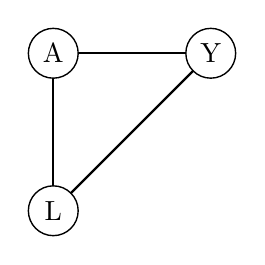
\begin{tikzpicture}
    \SetGraphUnit{2}
    \Vertex{A} \EA(A){Y} \SO(A){L}
    \Edges(L,A,Y)
    \Edges(L,Y)
  \end{tikzpicture}
  \hspace{5em}
  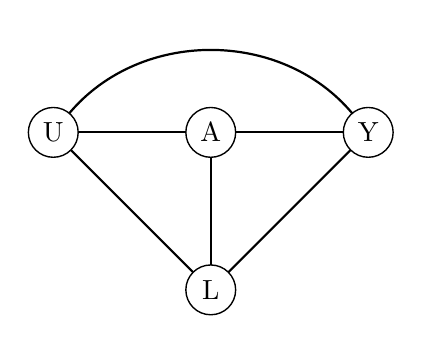
\begin{tikzpicture}
    \SetGraphUnit{2}
    \Vertex{A} \EA(A){Y} \SO(A){L} \WE(A){U}
    \Edges(L,A,Y)
    \Edges(L,Y)
    \Edges(U,L) \Edges(U,A)
    \tikzset{EdgeStyle/.append style = {bend left = 50}}
    \Edges(U,Y)
  \end{tikzpicture}
\end{center}

In reality, the graph on the right (where $U$ represents unmeasured values) is
more likely.  It is also likely that there are more $U$-like values, each
pointing to a subset of the available nodes.  The difficulty of working with
such an ambiguous graph is what leads to the decision to use the graph on the
left.

\section{Analysis} %%%%%%%%%%%%%%%%%%%%%%%%%%%%%%%%%%%%%%%%%%%%%%%%

The code for this report was written in Python with Pandas and the
causalinference package (available via pip).

Due to computational limitations, instead of using the full eleven-million rows
for computation, only a random subset was used.  This subset was drawn with
replacement from the full set of rows and contains ten thousand rows.

For this report, we restrict the analysis to the US site and ignore the others,
in order to limit the modification of the effect caused by the different users
of the different sites.  As described above, we only use eleven columns from the
initial dataset, and assume that they suffice to give conditional
exchangeability, as unlikely as that may be.  We use this to compute the
following: general summary statistics (as a baseline/reference against which to
compare the more advanced techniques that follow); an ordinary linear
least-squares estimate (to find the average treatment effect for each of the
treated and the controls); propensity scores (including a few quadratic terms
where $L_i\times L_j$), which are used for future analyses; stratification by
those propensity scores; and finally an estimate (using matching) of
the effect of mobile phone usage on booking.

\subsection{Summary statistics}

As mentioned above, these were only computed to serve as reference, and to show
whether controlling for $L$ (as the next subsections do) made a difference.
These statistics include the mean and standard deviation of each of the treated
and controls, as well as of each element of $L$, also split by treatment.

\subsection{Least-squares}

In an attempt to improve upon the results of the summary statistics above, a
linear least-square model was fit to the sampled data.  While this does not make
complete sense for all eleven members of $L$, it does for most of them.

For example, on the Expedia website, several search fields (including the number
of adults, children, and rooms) are pre-filled, and are filled with low values.
Any value greater than these defaults suggests that someone manually changed
them, thus making that person more likely to want to actually book a room
instead of just looking at what is available.  The Expedia mobile site does not
make this any harder or easier than the normal website does, so the impact there
should be minimal.

As another example, star ratings are integers between zero and five, inclusive.
A rating of zero means that no data are available.  Since better-rated hotels
are more likely to attract lookers and bookers than low-ranking (or unranked)
hotels, this also makes sense to be linear.

In contrast, hotel characteristics (the aforementioned ``bands'' estimated by
Expedia) are more of a mixed bag.  While popularity trivially is associated with
looking and booking (by definition), distance may not be as useful; an increase
in distance is not expected to increase nor decrease looking and booking rates,
nor to influence whether a user would choose to view it via a phone or via a
desktop/laptop web browser.  However, since a flat line (expected) is still a
line, it was included anyways.

\subsection{Propensity scores}

Due to the high dimensionality of $L$, as well as the diversity of entries that
it contains, any direct usage would likely violate positivity in some fashion.
While the eleven columns were chosen to lessen this likelihood, there are still
thousands of distinct possible values for any given row's $\vec{l}$, so a scalar
mapping such as what propensity scores provide is viable, useful, and what was
ultimately used.

\subsection{Stratification}

The propensity values from the previous subsection are used here for separation
into strata.  Values below about 10\% or above about 90\% were discarded to
avoid outliers.  Most propensity scores were fairly low ($<30\%$), with a few
high ones, so bins of equal size were not used.  Rather, an adaptive method is
used that recursively halves the sample until doing so stops providing
significantly useful information.

\subsection{Matching}

Separately from the computation of the stratification and propensity scores, a
matching procedure was used.  Matching was chosen because it should help avoid
the misleadingly-overrepresented rows where $Y=1$ (where people made bookings).
Each row where $A=1$ (mobile pageview) was matched with the desktop pageview
($A=0$) whose $\vec{l}$ was closest to it, where ``closest'' here means
minimizing the Euclidean distance ($L_2$ norm).  This way, rows with identical
$\vec{l}$ values are matched, and rows with similar-but-not-identical values can
still be kept.  There were more desktop pageviews than mobile pageviews, so the
leftover desktop data were not used for matching.  Matching also ensures
positivity, further increasing its usefulness for high-dimensional $L$.

\section{Results} %%%%%%%%%%%%%%%%%%%%%%%%%%%%%%%%%%%%%%%%%%%%%%%%%%%%%%%%%%%%%%

In general, this was a null result.  Users of Expedia.com are about as likely to
book a hotel when viewing hotel listings from their phones as they are when
viewing those same listings from their desktops and laptops.  Below are the
results of each test.

\subsection{Summary statistics}

Na\"{\i}vely, there was no meaningful difference between the means of the mobile
viewers and of the desktop viewers, at only 1.3\% (8.9\% of desktop users booked
versus 7.6\% of mobile users).  Among the means of each element of $L$, the
largest difference was for the same-country-or-not column, whose normalized
difference was 36\% (mobile users tended to choose the same country more often),
followed by the duration column, whose normalized difference was -20\% (desktop
users tended to pick slightly longer stays).  Again, these values do not adjust
for $L$, and should be treated as background.  Incidentally, the minute
difference in the booking rates is what prompted the selection of $A$ and $Y$
for this report.

\subsection{Least-squares}

Here, the results were also underwhelming.  The difference between the ATC
(desktop users) and ATT (mobile users) was minimal, with 95\% confidence
intervals that mostly overlapped --- over half of each interval fit inside the
other.  Thus, the conclusion at the head of this section is supported.

\subsection{Propensity scores and stratification}

The results of the stratification can be seen below.  The propensities were
chosen based on likelihood ratios, and include both linear and quadratic
($L_i\times L_j$, where $i,j$ were not always different) terms.  Computing the
same ATC and ATT for each stratum resulted in the same conclusion as above: even
when controlling for the confounding effect of $L$, phone usage does not tell us
much (if anything) about likelihood of booking.  Thus, the conclusion at the
head of this section is supported.

{
  \footnotesize
\begin{tabular}{llllllll}
  &
  \multicolumn{2}{l}{Propensity Score} &
  \multicolumn{2}{l}{Sample Size} &
  \multicolumn{2}{l}{Avg. Propensity} &
  Outcome\\
  Stratum & Min. & Max. & Desktop & Mobile & Desktop & Mobile & Raw-diff \\
  \hline
  1 & 0.087 & 0.107 & 295 & 21 & 0.098 & 0.100 & -0.037 \\
  2 & 0.107 & 0.119 & 270 & 43 & 0.113 & 0.113 & -0.084 \\
  3 & 0.119 & 0.135 & 541 & 84 & 0.127 & 0.128 & -0.060 \\
  4 & 0.135 & 0.156 & 1059 & 194 & 0.146 & 0.147 & -0.031 \\
  5 & 0.156 & 0.225 & 2017 & 419 & 0.185 & 0.185 & -0.012 \\
  6 & 0.225 & 0.276 & 936 & 302 & 0.253 & 0.254 & -0.010 \\
  7 & 0.277 & 0.299 & 893 & 393 & 0.290 & 0.290 & -0.052 \\
  8 & 0.300 & 0.318 & 834 & 351 & 0.310 & 0.310 & 0.004 \\
  9 & 0.318 & 0.904 & 791 & 440 & 0.337 & 0.339 & 0.011 \\
\end{tabular}
}

\subsection{Matching}

As with the other tests, matching also revealed minimal differences.  The
average effects in mobile users and in desktop users were -0.019 and -0.012,
respectively, and the standard deviation of both was 0.011.  While this makes
the causal booking ratio look high, the difference is not, just like in the case
of least-squares.  Thus, the conclusion at the head of this section is
supported.

%% Do not touch.
\printbibliography

\end{document}

Your proposal should describe a particular causal inference problem you will
investigate, one or more data sets you intend to analyze, the causal effect
measures you will use, a preliminary causal graph, and the analysis
techniques (e.g., matching, regression, etc.) you are thinking of using.

Not all data sets are suitable for causal inference.  You need to verify that
(conditional) exhangeability, positivity and well-defined interventions are at
least plausible for chosen variables in the data set.

You should prepare a 6-10 page report describing the problem, data sets,
analysis, and results in detail.  It is due the last day of classes.

%%%%%%%%%%%%%%%%%%%%%%%%%%%%%%%%%%%%%%%%%%%%%%%%%%%%%%%%%%%%%%%%%%%%%%%%%%%%%%%%

What if used Expedia/Datafest set? (observational)

Note: Expedia included too many booked=1 rows to boost their numbers (``trade secret'')
A = mobile or not
Y = booked or not (careful!)
L = everything else (limit to subset for sake of positivity)

``Did accessing Expedia via a phone make users more/less likely to book than via
a desktop?''

Conditional exchangeability: phones are popular these days, some sync tabs
Well-defined interventions: site has a mobile version, keyboard vs idle
browsing, ``seriousness''

L = these:
user_location_country == hotel_country
is_package
srch_co - srch_ci
srch_adults_cnt
srch_children_cnt
srch_rm_cnt
prop_is_branded
prop_starrating
distance_band
hist_price_band
popularity_band

Graph: counfounding
